\documentclass{beamer}

% -----------General Settings ------------
\usetheme{default}
\usetheme{Antibes}
\usecolortheme{dolphin}
\setbeamercolor{normal text}{bg=blue!3}
\beamertemplatetransparentcovereddynamicmedium
\beamertemplateshadingbackground{blue!4}{black!8}
\graphicspath{{./images/}} %images path
\title[Image Processing to Detect Worms]{Image Processing to Detect Worms}
\author[Javier Fern\'andez]{Javier Fern\'andez}
\institute[Uppsala University]{Uppsala University. Uppsala, Sweden}

\begin{document}
\maketitle

%----------- Introduction ----------------

\section{Introduction}
\subsection{C.elegans}

\begin{frame}{Caenorhabditis elegans (C.elegans)}

\begin{itemize}
  \item itemized item 1 \pause 
  \item itemized item 2 \pause
  \item itemized item 3
\end{itemize}

\end{frame}

\subsection{Motivation}
\begin{frame}{The problem: Motivation}

\begin{itemize}
  \item itemized item 1 
  \item itemized item 2 
  \item itemized item 3
\end{itemize}

\end{frame}
\subsection{Purpose}
\begin{frame}{The problem: Purpose}

\begin{itemize}
  \item itemized item 1 
  \item itemized item 2 
  \item itemized item 3
\end{itemize}

\end{frame}

\subsection{Background}
\begin{frame}{Background on Worm Detection}

\begin{itemize}
  \item itemized item 1 
  \item itemized item 2 
  \item itemized item 3
\end{itemize}

\end{frame}

% -----------------------------------------

\subsection{Objectives}
\begin{frame}{Objectives}

\large \textbf{General Objective}\\
\vskip7pt

\begin{itemize}
  \item itemized item 1 \pause 
\end{itemize}

\vskip7pt
\pause \large \textbf{Specific Objectives}\\
\vskip7pt

\begin{itemize}
  \item itemized item 1 \pause 
  \item itemized item 2 \pause
  \item itemized item 3
\end{itemize}

\end{frame}

%-----------------------------------------

\section{Methodology}
\subsection{Solution Methodology Flowchart}
\begin{frame}{}

\begin{figure}[h t b p ! H]
 \centering
   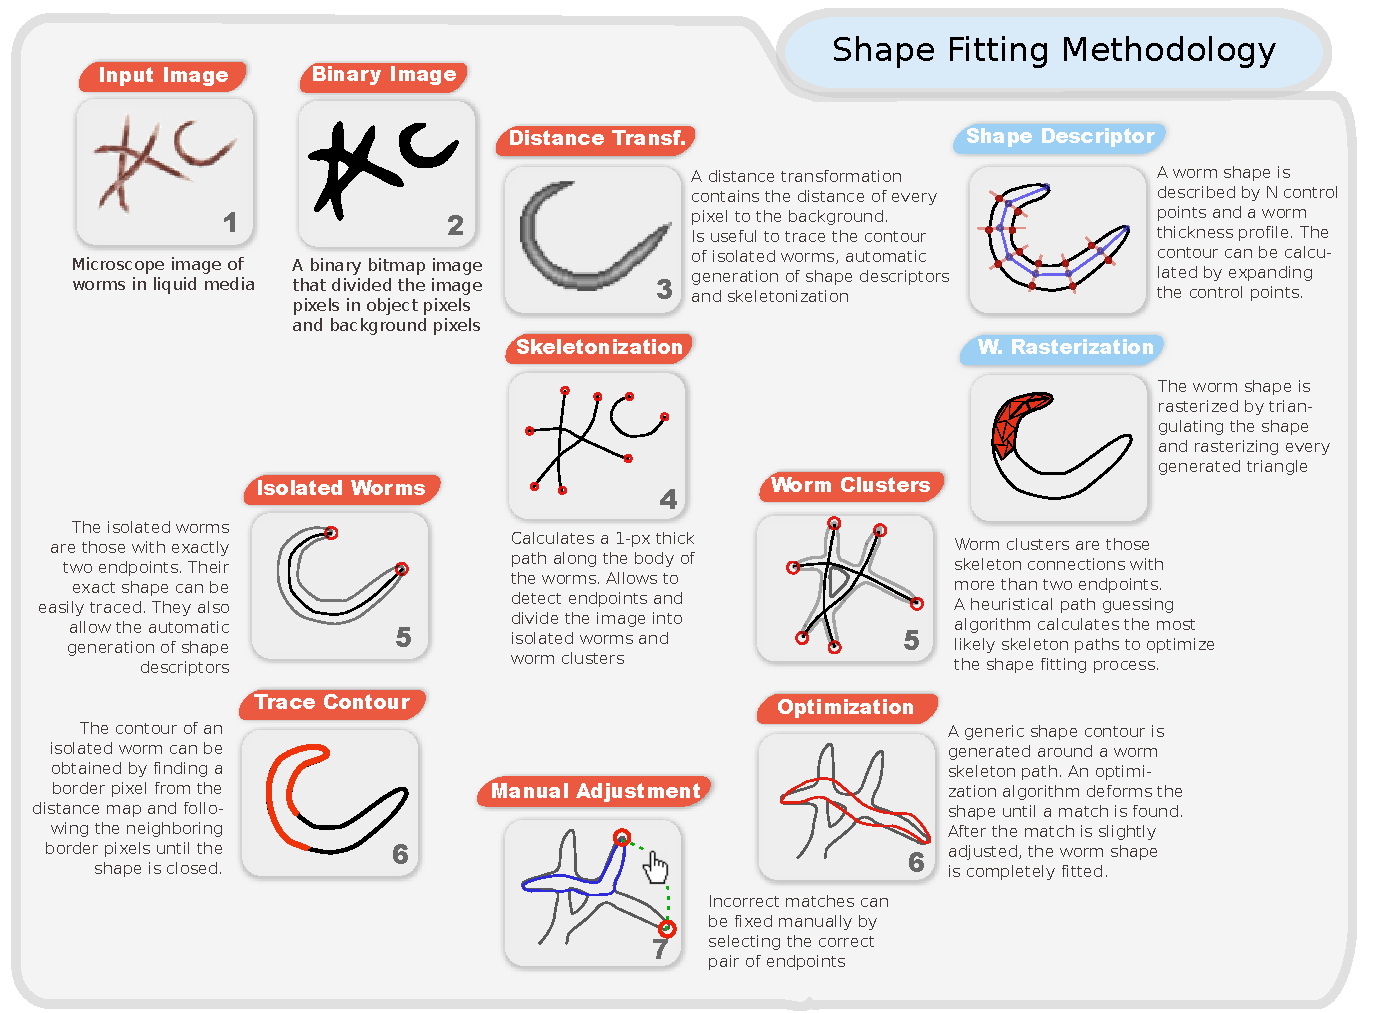
\includegraphics[scale=0.46]{diagrams/design.pdf}
\end{figure}
\end{frame}


% -------- Original and Thresholding -----------

\subsection{Thresholding}
\begin{frame}{Thresholding}

\begin{columns}[c]
\column{1.5in}
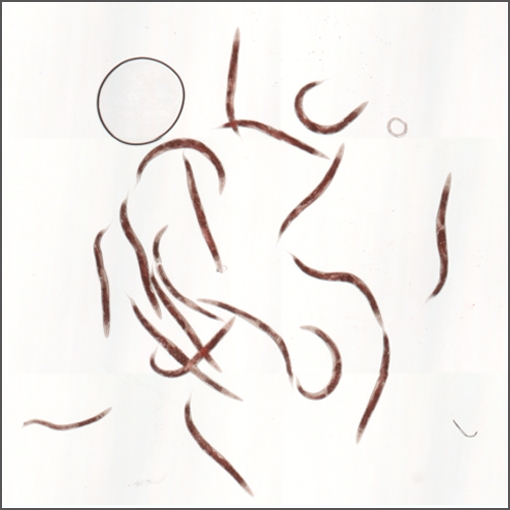
\includegraphics[scale=0.27]{original}
\column{1.5in}
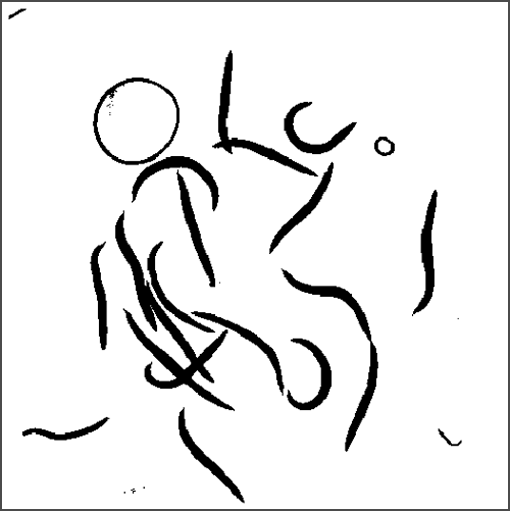
\includegraphics[scale=0.27]{thres/worms}

\end{columns}

\end{frame}

% -------- Distance Transformation  -----------

\subsection{Distance Transformation}
\begin{frame}{Distance Transformation: Manhattan Distance}

\begin{columns}[c]
\column{2.4in}
\begin{itemize}
\item Improve skeletonization algorithm \pause
\item Trace contour of isolated worms \pause
\item Automatic calculation of worm profile \pause
\item Path guessing algorithm
\end{itemize}
\column{2in}
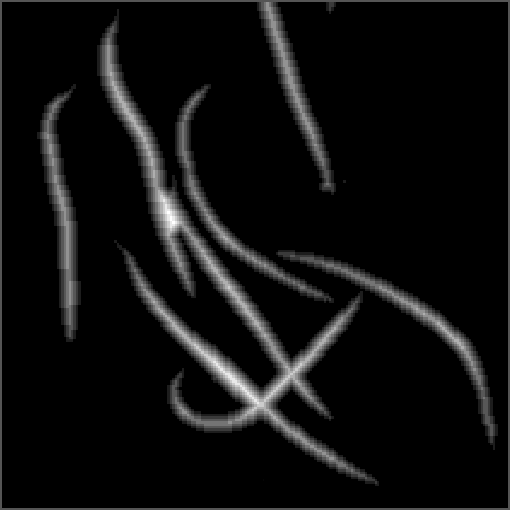
\includegraphics[scale=0.27]{results/test1/dt-shape1}

\end{columns}

\end{frame}


% -------- Skeletonization  -----------

\subsection{Skeletonization}
\begin{frame}{Worm Skeletonization}

\begin{columns}[c]
\column{2.4in}
\begin{itemize}
\item Thinning Algorithm $+$ Distance Map \pause
\item 1 pixel thick paths that tend to the medial axes \pause
\item Skeleton endpoint expansion and Worm Endpoint detection \pause
\item Segmentation in groups
\end{itemize}
\column{2in}
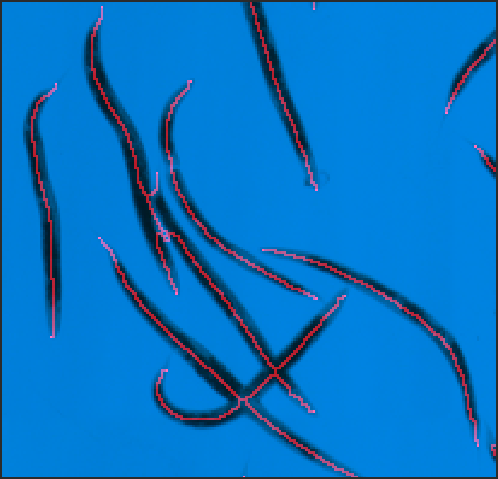
\includegraphics[scale=0.3]{skeleton1}

\end{columns}

\end{frame}


% -------- Shape Matching  -----------

\subsection{Shape Fitting}
\begin{frame}{Isolated Worms}

\begin{columns}[c]
\column{2.4in}
\begin{itemize}
\item Contour can be traced easily.The shape is rasterized 
and thus fitted \pause
\item Worm Profiling 
\end{itemize}
\column{2.2in}
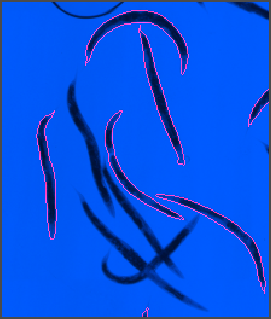
\includegraphics[scale=0.5]{iso}
\end{columns}

\end{frame}

%------------------------------------------




\end{document}